\section{Como correr o programa}

\subsection{Módulos}
\par Antes de podermos correr o programa precisamos de ter os módulos requiridos pelo mesmo instalados. Para instalar os módulos necessários pode-se utilizar uma ferramenta chamada \textit{cpanm}\cite{cpanm}. Pode-se descarregar esta ferramenta para linux com o comando de terminal \textit{sudo apt install cpanminus}.\newline
Após instalar a ferramenta deve-se garantir que se têm os seguintes módulos instalados\footnote{Nota: Para descarregar os módulos use no terminal o comando cpanm install 'nome do módulo'}:

\begin{enumerate}
	\item Crypt::OpenSSL::X509
	\item DateTime
	\item Digest::SHA
	\item MIME::Base64
	\item Getopt::Long
	\item POSIX
	\item List::MoreUtils
	\item Carp
	\item FindBin
	\item IO::Prompt
	\item REST::Client
	\item XML::Compile::WSDL11
	\item XML::Compile::SOAP11
	\item XML::Compile::Transport::SOAPHTTP
	\item Encode
	\item Bit::Vector
	\item HTTP::Request
	\item HTTP::Parser
	\item Log::Log4perl
	\item LWP::ConsoleLogger
	\item strict
\end{enumerate}

Agora que temos os módulos necessários instalados podemos correr o programa e para  o fazer temos várias opções. Para saber qual a sintaxe pela qual o programa se rege deve-se chamar o programa seguido do argumento -h:
\begin{itemize}
	\item perl signpdf\_cli.pl -h
\end{itemize} 
\hfill\newline
O programa requer sempre 3 inputs obrigatórios:
\begin{itemize}
	\item Número de telemóvel do utilizador
	\item Pin da chave móvel digital
	\item Nome do pdf a assinar
\end{itemize}
\hfill\newline
Adicionalmente o programa permite ao utilizador fornecer 2 inputs extra \textit{Output file} e \textit{Datetime} que são respetivamente o nome a ser atribuido ao pdf assinado e a data a usar para assinar o mesmo, podendo o utilizador escolher fornecer apenas o primeiro, apenas o segundo ou ambos.\newline
Assim, apresentam-se em seguida as várias combinações disponíveis para a utilização da app:
\begin{enumerate}
	\item perl signpdf\_cli.pl -u '+351 XXXXXXXXX' -p XXXX -infile 'nome do ficheiro'.pdf
	\item perl signpdf\_cli.pl -u '+351 XXXXXXXXX' -p XXXX -infile 'nome do ficheiro'.pdf - outputfile 'nome do ficheiro'.pdf
	\item perl signpdf\_cli.pl -u '+351 XXXXXXXXX' -p XXXX -infile 'nome do ficheiro'.pdf -datetime YYYY-MM-DDTHH:MM:SS.SSSSSS
	\item perl signpdf\_cli.pl -u '+351 XXXXXXXXX' -p XXXX -infile 'nome do ficheiro'.pdf - outputfile 'nome do ficheiro'.pdf -datetime YYYY-MM-DDTHH:MM:SS.SSSSSS
\end{enumerate}


Caso corra a aplicação como um utilizador regular (sem debug) o resultado esperado é o seguinte:
\begin{figure}[H]

  \centering
  \captionsetup{justification=centering}

  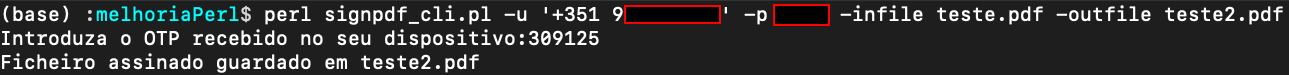
\includegraphics[scale = 0.25]{resultado1.png}
  
  \caption {Resultado de correr o programa sem o modo debug}

\end{figure}


 Caso corra a aplicação em modo debug poderá ver a forma dos envelopes enviados bem como a informação que circula nos seus headers e os seus conteúdos, o resultado esperado é o seguinte:

\begin{figure}[H]

  \centering
  \captionsetup{justification=centering}

  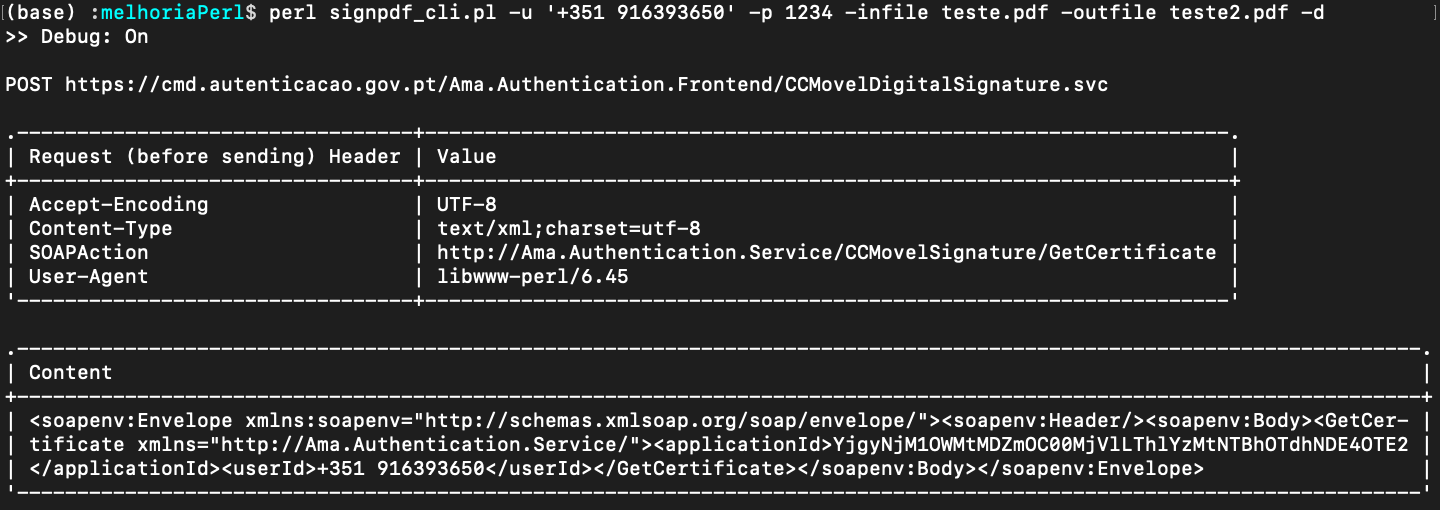
\includegraphics[scale = 0.25]{resultado2.png}
  
  \caption {Resultado de correr o programa com o modo debug}

\end{figure}
\newpage
\subsection{Replicação de testes}

Caso se pretendam replicar os testes realizados sobre a aplicação é necessário instalar alguns programas bem como alguns módulos do perl. Os módulos a instalar são os seguintes:

\begin{enumerate}
	\item Devel::Cover
	\item Perl::Critic
	\item Test::Vars
	\item Test::LectroTest
\end{enumerate}
Igualmente é necessário instalar os seguintes programas e bibliotecas (os links para obter os elementos listados também são fornecidos). Cada um dos elementos possui documentação para auxiliar a sua instalação e configuração:
\begin{enumerate}
	\item SonarQube (sonarqube.org)
	\item Biblioteca Perl para o SonarQube (https://github.com/sonar-perl/sonar-perl)
	\item Sonar-Scanner para o SonarQube (https://docs.sonarqube.org/latest/analysis/scan/sonarscanner/)
\end{enumerate}

Após a instalação dos recursos supramencionados basta analisar o programa criado com os mesmos, seguindo os passos referidos na \autoref{sec:Testes}.




